\section{Analysis}
\label{sec:analysis}

\noindent
Sec.~\ref{sec:low-resource-nonen}에서 우리는 특정 언어 조합들, 예를 들어 라오어--태국어, 바스크어--한국어, 아르메니아어--한국어가 영어 skeleton 기반 추론보다 높은 성능을 보일 수 있음을 관찰하였다. 그러나 정량 결과만으로는 이러한 이득의 원인을 단정하기 어렵다. 본 절에서는 LLM-as-a-Judge 기반 정성 평가를 통해 skeleton generation quality가 이러한 효과를 충분히 설명할 수 있는 요인인지 검토한다. 평가 방법론은 Appendix~\ref{Appendix:skeleton_qualitative}에 제시한다.

\begin{figure}[!t]    
    \centering
    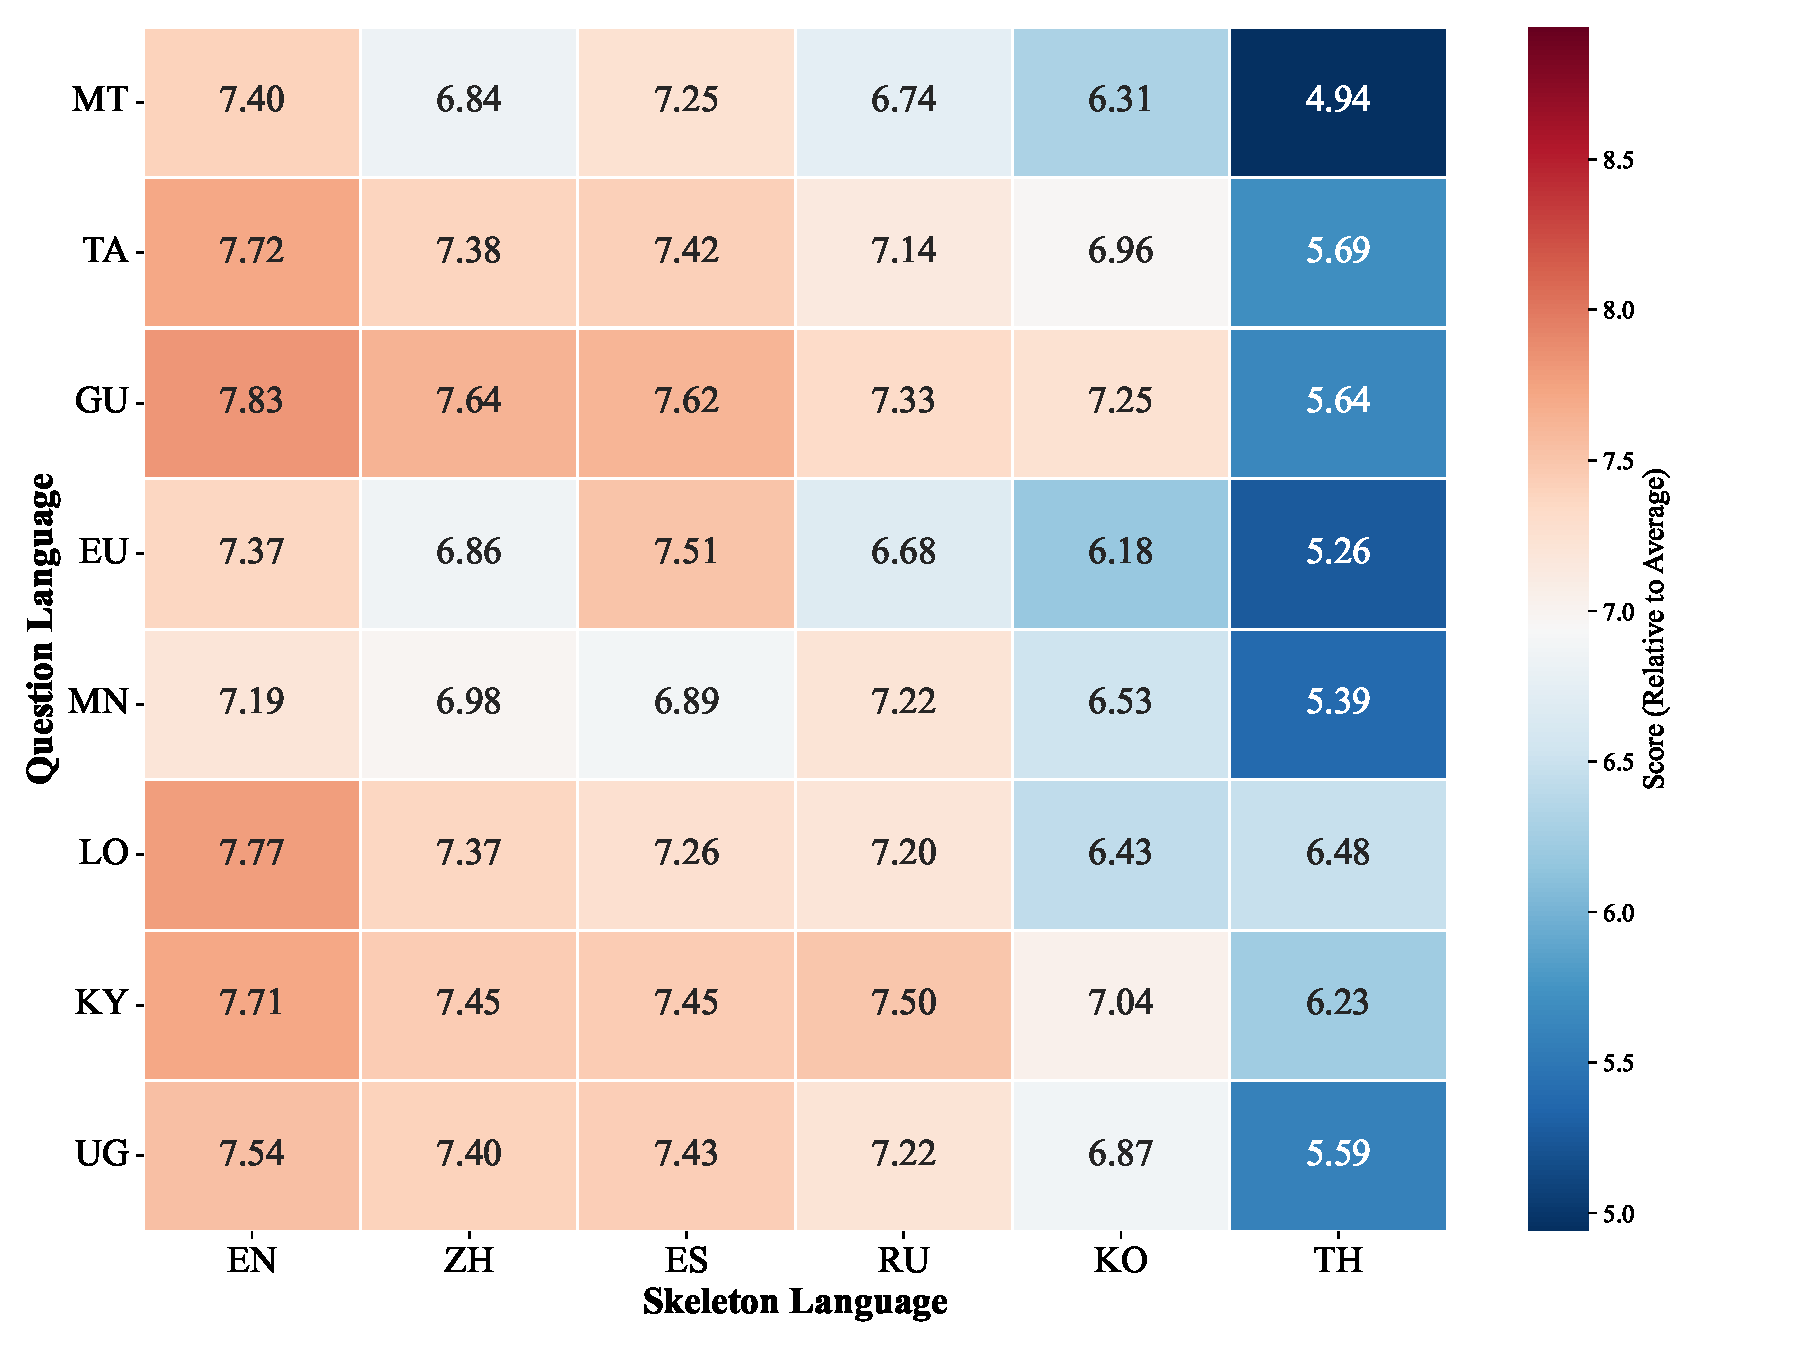
\includegraphics[width=\columnwidth]{Figures/Images/lang_pair_heatmap_styled.pdf}
    % 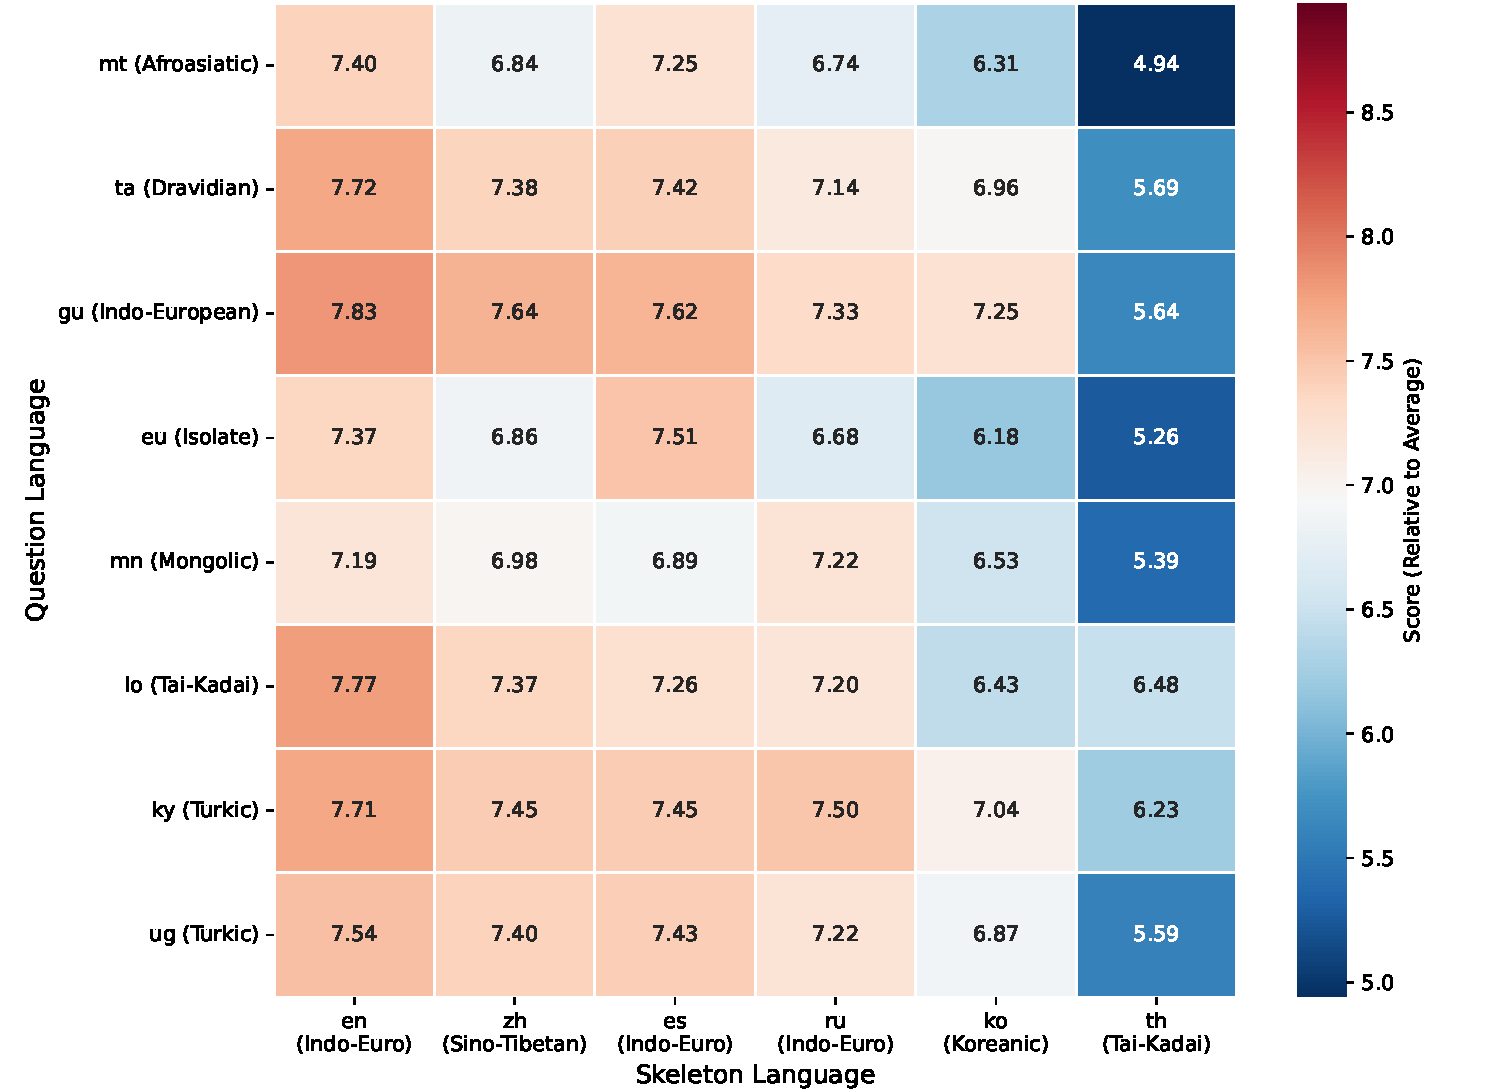
\includegraphics[width=\columnwidth]{Figures/Images/lang_pair_heatmap_cropped.pdf}
    \caption{\small Skeleton quality heatmap across language pairs. English skeletons yield highest quality (7.57), while Thai performs worst (5.65).}
    
\label{fig:lang_pair_heatmap}
    \vspace{-0.15in}
\end{figure}
\begin{figure}[!ht]    
    \centering
    % 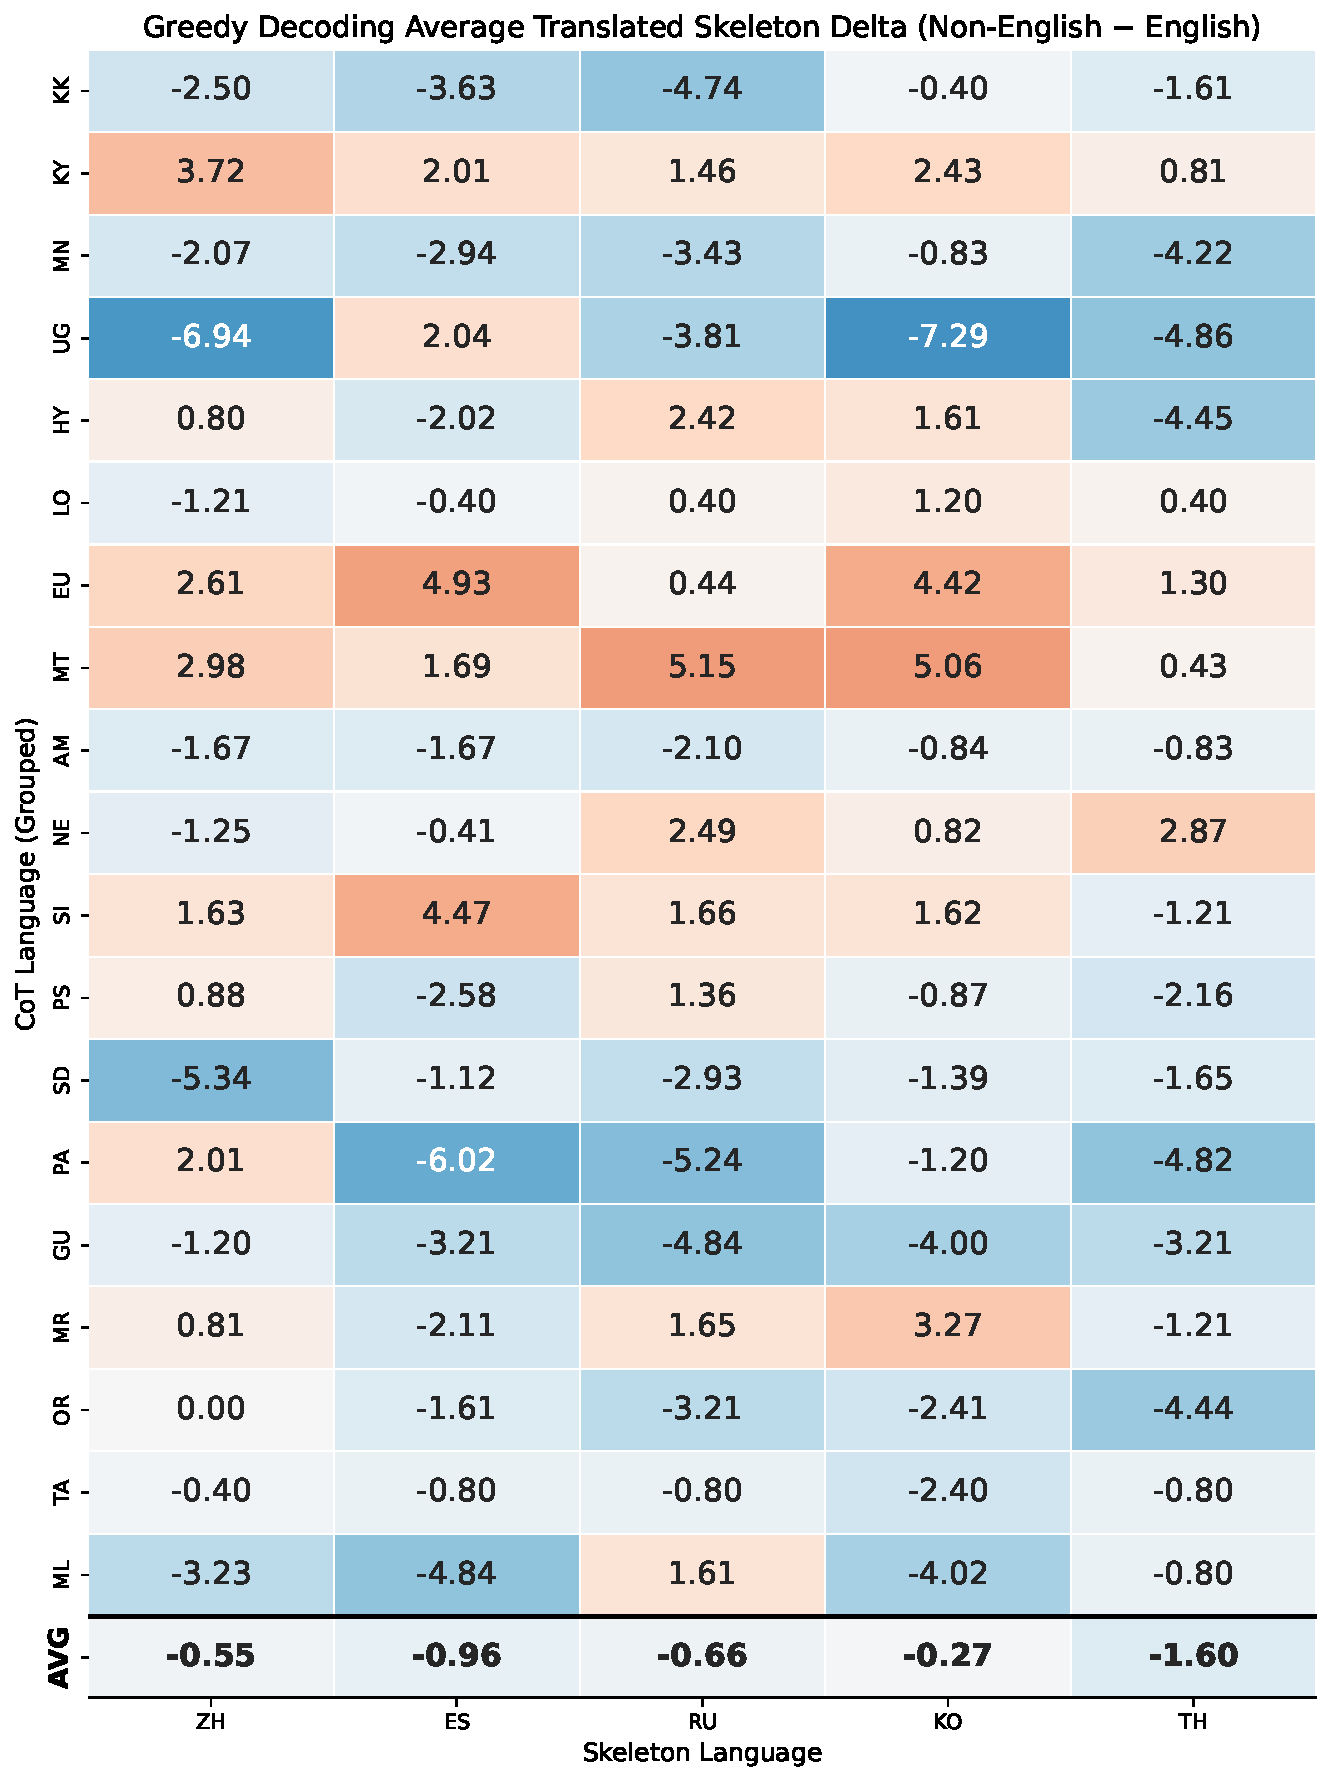
\includegraphics[width=\columnwidth]{Figures/Images/trans.pdf}
    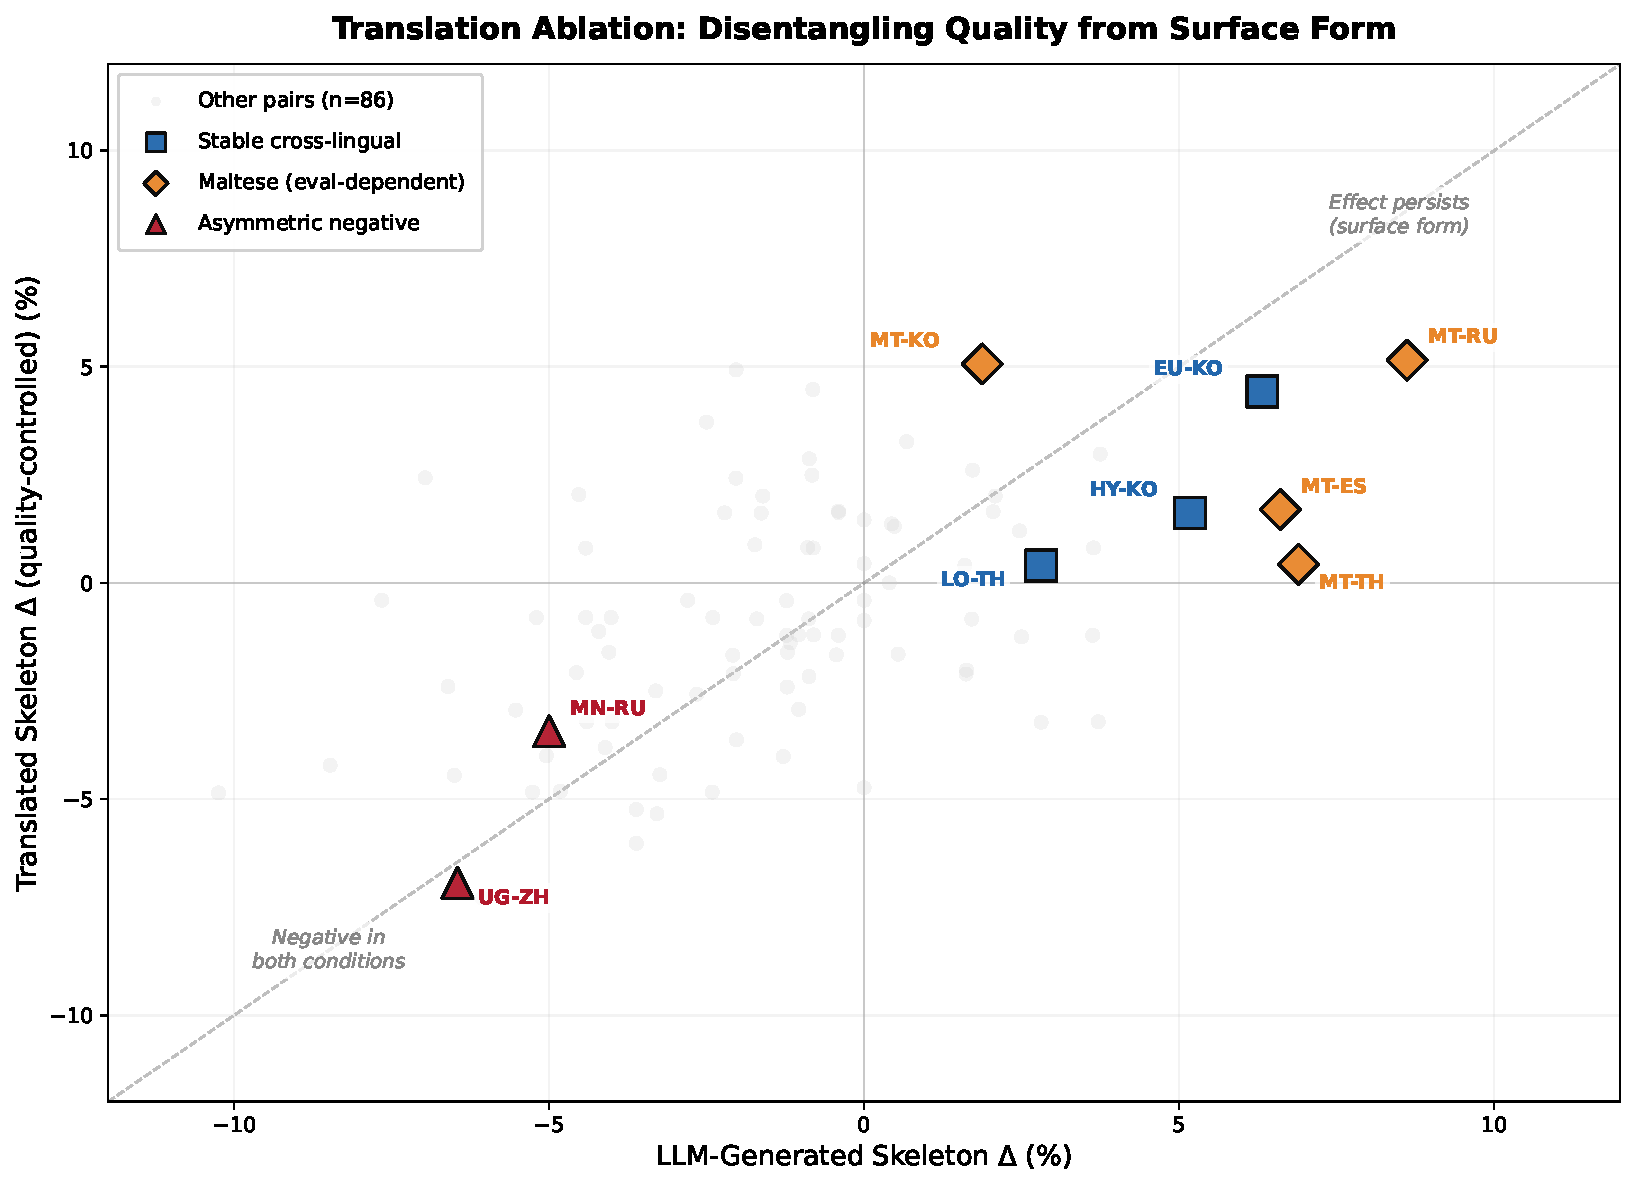
\includegraphics[width=\columnwidth]{Figures/Images/analysis_scatter_ablation.pdf}
    \caption{\small Translation ablation results. Each point is a (target, skeleton) pair, with $\Delta$ from LLM-generated skeletons on the x-axis and translated skeletons on the y-axis. Points near the diagonal indicate effects robust to skeleton quality.}
    \label{fig:translation_scatter}
    \vspace{-0.15in}
\end{figure}

\paragraph{Dominance of English Quality.}
Fig.~\ref{fig:lang_pair_heatmap}에서 보이듯, 영어는 가장 높은 intrinsic skeleton quality 점수($7.57$)를 기록하며, 그다음으로 스페인어($7.35$), 중국어($7.24$), 러시아어($7.13$)가 뒤따른다. 반면 한국어($6.69$)와 태국어($5.65$)는 상대적으로 낮은 점수를 보인다. 이는 풍부한 사전학습 데이터의 영향을 받는 영어가 skeleton generation quality 측면에서 가장 안정적인 기반을 제공함을 시사하며, 앞선 절에서 영어 skeleton이 다수 target language에 대해 안정적인 기본 선택지로 작용한 관찰과도 일관된다.

\paragraph{Quality Alone Does Not Predict Performance.}
그러나 skeleton quality가 downstream reasoning performance와 단순히 비례하는 것은 아니다. 라오어(lo)의 경우, 태국어 skeleton의 quality score($6.48$)는 영어 skeleton($7.77$)보다 $1.29$점 낮지만, Fig.~\ref{fig:heatmap-greedy}에서 태국어 skeleton은 영어 skeleton 대비 $+2.81$의 성능 향상을 보인다. 마찬가지로 바스크어(eu)의 경우, 한국어 skeleton은 영어 skeleton보다 낮은 quality score를 보이지만($6.18$ vs. $7.37$), greedy decoding에서는 $+6.32$의 성능 향상을 가져온다. 반대로, surface-level affinity만 존재하는 일부 경우에는 skeleton quality가 비슷하거나 더 높음에도 성능이 크게 하락한다. 예를 들어 위구르어--중국어는 quality score가 유사하지만($7.40$ vs. $7.54$), 성능은 $-6.45$ 하락하며, 몽골어--러시아어는 러시아어 skeleton의 quality가 영어보다 약간 높음에도($7.22$ vs. $7.19$) $-5.00$의 성능 하락을 보인다. 이러한 비대칭적 양상은 skeleton effectiveness가 generation quality만으로 설명될 수 없음을 시사한다.

\paragraph{Implication.}
종합하면, skeleton quality는 비영어 skeleton 효과를 설명하는 단일한 충분 요인이 아니다. 더 낮은 quality를 가진 비영어 skeleton이 영어 skeleton보다 높은 성능을 보이는 사례와, 비슷한 quality를 가진 skeleton이 크게 낮은 성능을 보이는 사례가 함께 존재한다는 점은 추가적인 요인이 개입하고 있음을 보여준다. 또한 Sec.~\ref{sec:low-resource-nonen}에서 논의했듯, 일부 cell은 evaluation protocol에 따라 effect size가 달라지는 양상을 보인다. 따라서 우리는 skeleton-language effect를 (i) generation quality, (ii) 잠재적인 cross-lingual alignment 요인, 그리고 (iii) evaluation protocol의 sampling 특성이 상호작용한 결과로 해석한다. 이러한 복합적인 양상은 단일 quality metric이나 단일 evaluation setting만으로 식별하기 어렵기 때문에, \Lasef의 다층적 탐색 framework가 필요함을 뒷받침한다.